\section{}
\label{sec:p1}
%%%%%%%%%%%%%%%%%%%%%%%%%%%%%%%%%%%%%%%%%%%%%%%%%%%%%%%%%%%%%%%%%%%%%%
\paragraph{a)}
The '\textit{seismic.dat}' data contains seismic data on a regular grid $(75\times75)$, $L_D$, denoted as $\{d(\vect{x}) \ssep \vect{x}\in L_D\} \ssep d(\vect{x})\in \R$, and visually represented by the map in Figure \ref{fig:data}.
The seismic data has the likelihood model given by the equation
\begin{equation}
    [d_i\given\vect{l}] = \begin{cases}
                                0.02 + U_i, & l_i = 0 \Rightarrow \mathrm{sand} \\
                                0.08 + U_i, & l_i = 1 \Rightarrow \mathrm{shale}
                             \end{cases}
                            , i = 1, 2, ..., n,
    \label{eq:likelihood}
\end{equation}

where $U_i \overset{\mathrm{iid}}{\sim}\N\{0,0.06^2\}$. This means that we can rewrite Equation \ref{eq:likelihood} to 
\begin{equation}
    [d_i\given\vect{l}] = \begin{cases}
                                A_i\overset{\mathrm{iid}}{\sim}\N\{0.02,0.06^2\}, & l_i = 0 \Rightarrow \mathrm{sand} \\
                                B_i\overset{\mathrm{iid}}{\sim}\N\{0.08,0.06^2\}, & l_i = 1 \Rightarrow \mathrm{shale}
                             \end{cases}
                            , i = 1, 2, ..., n.
    \label{eq:likelihood2}
\end{equation}
The likelihood model $p(\vect{d}\given \vect{l})$ is then given by 
\begin{equation}
    \begin{array}{rcl}
        [\vect{d}\given\vect{l}] \sim p(\vect{d}\given\vect{l}) & = & \prod\limits_{i=1}^n p(d_i\given l_i) \\
        & = & (0.0072\pi)^{-n/2} \prod\limits_{i=1}^n l_i \exp\left\{\frac{(d_i - 0.08)^2}{0.0072} \right\} + (1-l_i) \exp\left\{\frac{(d_i - 0.02)^2}{0.0072} \right\} \\
         & = & (0.0072\pi)^{-n/2} \exp\left\{\frac{1}{0.0072} \left[\sum\limits_{i \st l_i = 0} (d_i - 0.02)^2 + \sum\limits_{i \st l_i = 1} (d_i - 0.08)^2\right]\right\} \, .
    \end{array}
    \label{eq:likelihood3}
\end{equation}

\begin{figure}
    \centering
    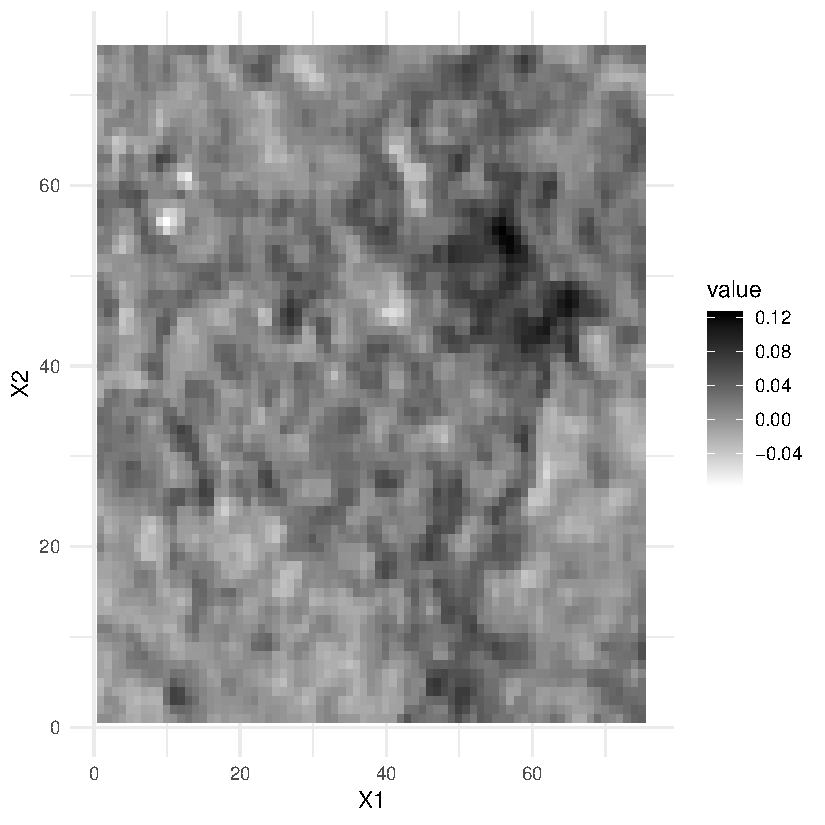
\includegraphics[scale=0.95]{figures/seismic_data.pdf}
    \caption{Map of the seismic data $d(\vect{x})$ on a grid $\matr{L_D}$}
    \label{fig:data}
\end{figure}
%%%%%%%%%%%%%%%%%%%%%%%%%%%%%%%%%%%%%%%%%%%%%%%%%%%%%%%%%%%%%%%%%%%%%%
\paragraph{b)}
We consider a uniform form prior $\prob(\vect{l}) = const$. We have $\prob(\vect{l}) = \prod_{i=1}^n \prob(l_i)$ and $\prob(l_i) = 1/2$. Assuming the data are collected independently, i.e. $\prob(\vect{d}) = \prod_{i=1}^n \prob(d_i)$, we get the posterior
%
\begin{align*}
    \prob(\vect{l} \given \vect{d}) &= \frac{\prob(\vect{d} \given \vect{l}) \prob(\vect{l})}{\prob(\vect{d})} \\
    &= \prod_{i=1}^n \frac{\prob(d_i \given l_i) \prob(l_i)}{\prob(d_i)} \\
    &= \prod_{i=1}^n \prob(l_i \given d_i) \, ,
\end{align*}
%
where $\prob(d_i) = 1/2 \cdot [\prob(d_i \given l_i=0) + \prob(d_i \given l_i=1)]$. Thus the values of $l_i$, $i = 1, \dots, n$ are independent Bernoulli random variables with parameters $p_i = \prob(l_i \given d_i)$. The expectation of the $i$th element is $p_i$ and the variance is $p_i(1-p_i)$. 

\figref{fig:b_sims}, \figref{fig:b_mean} and \figref{fig:b_var} show 10 simulations from the posterior distribution, the posterior mean and the posterior variance, respectively. We see that the mean is high where the measurements are high and low where the measurements are low. The variance is low both where the measurements are high and low, while it is larger in ares where the measurements are not clearly indicating whether the is shale or sand in an area. The posterior mean $\E[\vect{l} | \vect{d}]$ is the probability that an area contains shale (1).

The maximum marginal posterior predictor $\text{MMAP}\left\{\vect{l}|\vect{d}\right\}$ is the vector of values maximizing $p(l_i \given d_i)$, $i = 1, \dots, n$, which are 1 where $p(l_i \given d_i) > 0.5$ and 0 else.

\begin{figure}
    \centering
    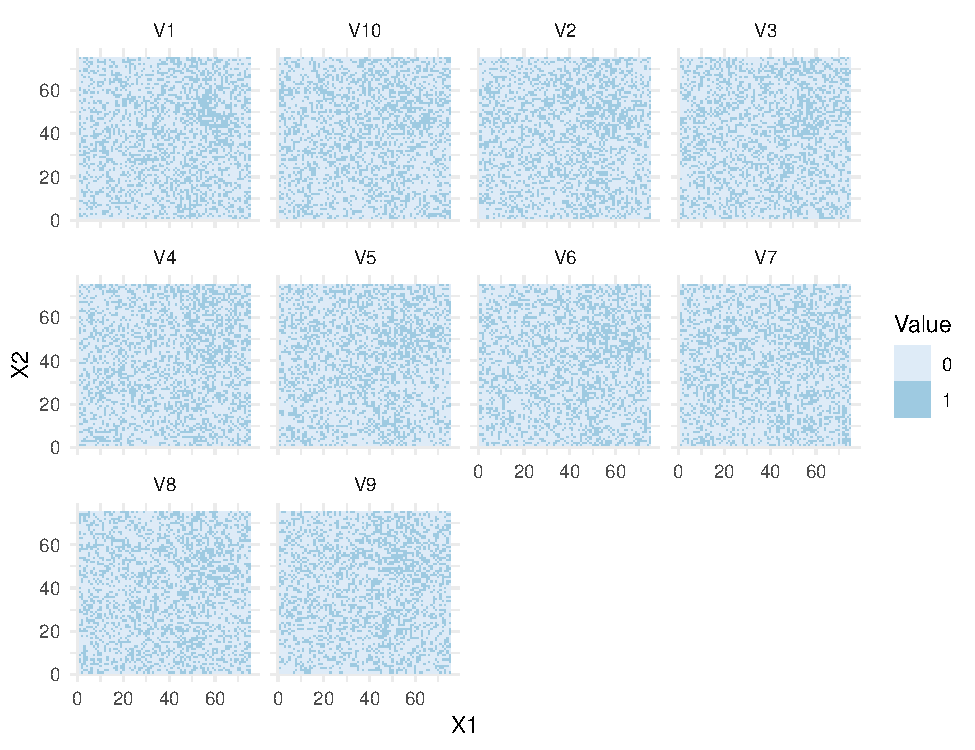
\includegraphics{figures/b_sims.pdf}
    \caption{10 simulations from the posterior given in b).}
    \label{fig:b_sims}
\end{figure}

\begin{figure}
    \centering
    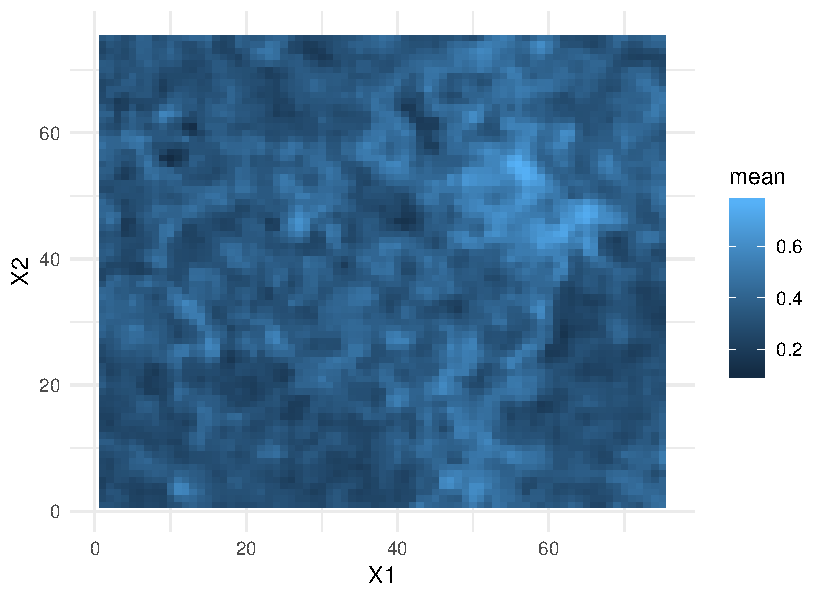
\includegraphics{figures/b_mean.pdf}
    \caption{Posterior mean as derived in b).}
    \label{fig:b_mean}
\end{figure}

\begin{figure}
    \centering
    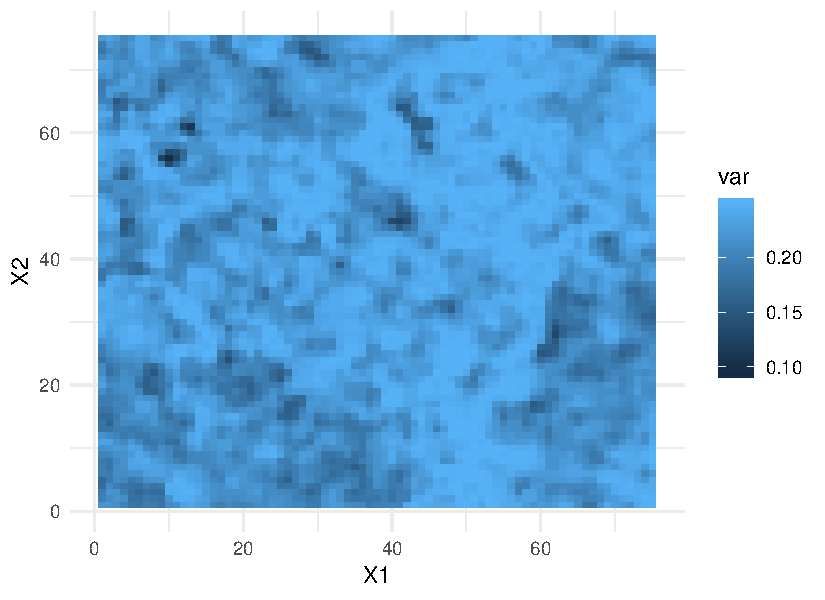
\includegraphics{figures/b_var.pdf}
    \caption{Posterior variance as derived in b).}
    \label{fig:b_var}
\end{figure}

%%%%%%%%%%%%%%%%%%%%%%%%%%%%%%%%%%%%%%%%%%%%%%%%%%%%%%%%%%%%%%%%%%%%%%
\paragraph{c)}


%%%%%%%%%%%%%%%%%%%%%%%%%%%%%%%%%%%%%%%%%%%%%%%%%%%%%%%%%%%%%%%%%%%%%%
\paragraph{d)}

